\chapter{Principal Component Analysis}
\label{ch-pca}


%https://en.wikipedia.org/wiki/Principal_component_analysis

%
%https://online.stat.psu.edu/stat508/lessons/Lesson07

This chapter is based on Ref.\cite{wiki-pca}.

{\bf Principal Component Analysis} (PCA)
is the most common way of doing 
{\bf Dimensionality Reduction} (See Chapter \ref{ch-dim-reduc})

\begin{itemize}


\item{\bf Notation}


$X=[x_1, x_2, \ldots, x_\calf]\in \RR^{N\times \calf}$ is the {\bf initial dataset} to be dimensionality reduced (i.e., the number of its  feature columns is to be reduced). Henceforth, we will assume that $X$ has {\it zero mean}. If $X$ doesn't have zero mean initially, 
replace $X_{\s, i}$ by 
$X_{\s, i}-\frac{1}{N}\sum_\s X_{\s, i} $


$Y=[y_1, y_2, \ldots, y_\calf]\in \RR^{N\times \calf}$. The $y_i$ for $i=1,2, \ldots, \calf$ are called the {\bf principal components} (PCs).

$U= [u_1, u_2, \ldots u_{N}]
\in\RR^{N \times N}$, $UU^T =U^TU =1$ ($U$ orthogonal). Components of
$u_\s$ will be denoted by $(u_\s)_{\s'}$
for $\s'=1,2, \ldots, N$.
 
$\Lam= \left[\begin{array}{c}
\Lam_D\\
0^{(N-\calf)\times \calf}
\end{array}\right]\in\RR^{N\times \calf}$, $\Lam_D=diag(\lam_1, \lam_2, \ldots, \lam_{\calf})$

$W= [w_1, w_2, \ldots w_{\calf}]\in\RR^{\calf\times \calf}$, $WW^T=W^TW=1$
($W$ orthogonal) Components of
$w_i$ will be denoted by $(w_i)_f$
for $f=1,2, \ldots, \calf$.

{\bf Singular Value Decomposition} (SVD)
\beqa X &=& U\Lam W^T
\\
&=& \sum_{f=1}^\calf \lam_f u_f w^T_f
\eeqa

\item {\bf Covariance Matrix}
\beqa
X^T X &=& W \Lam^T U^T U \Lam W^T
\\
&=& W \Lam^T \Lam W^T
\\
&=& W \Lam_D^2 W^T
\\
&=&
\sum_{f=1}^\calf \lam_f^2 w_f w_f^T
\eeqa
Reorder diagonal elements of $\Lam_D$
and columns of $W$ so that  
$\lam_1\geq \lam_2\geq \ldots\geq \lam_\calf$.

We will refer to $\lam_i^2$ 
as the ith {\bf principal value} (PV)
of X and to $w_i=[W_{r, i}]_{r=1}^\calf\in \RR^{\calf\times 1}$
as the ith {\bf principal axis} (PA) 
of $X$.

Note that
\beqa
Y &=& XW\\
&=& U\Lam W^T W
\\\
&=&
U \Lam 
\eeqa

$Y= U\Lam$ is called the {\bf Polar Decomposition} of $Y$.

Note that
\beq
Y_{\s, i} = \sum_j X_{\s, j}W_{j,i}=\sum_jU_{\s, j}\lam_{j}
\delta_{j,i} 
\eeq
so

\beq
y_i = Xw_i = u_i\lam_i
\eeq

Note that

\beqa
[Y^T Y]_{i,j}&=&Y_{\s, i} Y_{\s, j}
\\&=& 
y^T_iy_j
\\
&=&
\lam_i\lam_j u_i^T u_j
\\&=&
\lam_{i}^2\delta_{i,j}
\eeqa

\item {\bf Truncation}

Define $X_{\leq \Phi}$ by
\beq
X_{\leq \Phi} = U\Lam_{\leq \Phi}W^T
\label{eq-x-ulam-wt}
\eeq
where $\Lam_{\leq\Phi}= diag(\lam_1, \lam_2, \ldots, \lam_{\Phi}, 0^{\calf-\Phi})$.

Define $Y_{\leq \Phi}$ by

\beq
Y_{\s, i\leq \Phi} = \sum_j X_{\s, j}W_{j,i\leq \Phi}=U_{\s, i}\lam_{i\leq \Phi}
\eeq

\beqa
Y_{\leq \Phi} &=& XW_{\leq \Phi} = U\Lam_{\leq \Phi}
\\ &=& X_{\leq \Phi}W\;\;\text{(from Eq.(\ref{eq-x-ulam-wt}))}
\eeqa
Then

\beq
X-X_{\leq \Phi} = U(\Lam - \Lam_{\leq \Phi})W^T
\eeq


\beq
Y-Y_{\leq \Phi} = U(\Lam - \Lam_{\leq \Phi})
\eeq


\beqa
Error &=& \tr\left[(X-X_{\leq \Phi})^T(X-X_{\leq \Phi})\right]
\\
&=& \tr\left[(Y-Y_{\leq \Phi})^T(Y-Y_{\leq \Phi})\right]
\\
&=&
\tr\left[(\Lam - \Lam_{\leq \Phi})^2\right]
\\
&=&
\sum_{i=\Phi+1}^\calf \lam_i^2
\eeqa



\item{\bf PCA as solution to maximization problem}

Define the first PA $w_1$ by
\beqa
w_1&=&
\argmax_{w_1:\; w_1^Tw_1=1}
y_1^T y_1
\\
&=& 
\argmax_{w_1:\; w_1^Tw_1=1}
w_1^T X^T X w_1
\\
&=& \argmax_{w_1}\sum_\s
\frac{w_1^T X^T X w_1}{w_1^T w_1}
\eeqa

Consider the following 
diagonalization of $I_\calf$ (This is one of
many possible diagonalizations of $I_\calf$)
\footnote{In Quantum Mechanics,
$$\sum_i \ket{\phi_i}\bra{\phi_i}=1$$
is called a {\bf completeness condition} for an orthonormal basis $\{\ket{\phi_i}:i\}$.
{\bf Orthonormality} means $$\av{\phi_i|\phi_j}
=\delta_{i,j}$$.}
\beq
\sum_k w_k w^T_k = 1
\eeq
Multiplying both sides 
of this by $X$ on the left

\beq
X = \sum_{k=1}^{\calf}
\underbrace{\underbrace{X w_k}_{Y_k} w^T_k}_{X_k}
\eeq
Define $X^{\geq \Phi}$ by

\beqa
X^{\geq \Phi} &=& X -\sum_{k=1}^{\Phi-1}
\underbrace{X w_k w^T_k}_{X_k}
\\
&=&
\sum_{k=\Phi}^{\calf} X_k
\label{eq-X-super-f}
\eeqa
Multiplying $X^{\geq \Phi}$ on  the right
by $w_a$ gives

\beqa
\underbrace{X^{\geq \Phi} w_a}_{Y^{\geq \Phi}_a}&=& \underbrace{Xw_a}_{Y_a}
[1-\indi(a< \Phi)]
\\
&=&
Y_a\indi(a\geq \Phi)
\label{eq-Y-super-f}
\eeqa
See Fig.\ref{fig-XY-super-f}
for a pictorial
representation of Eqs.\ref{eq-X-super-f}
and \ref{eq-Y-super-f}.


Now we can define the $\Phi$'th
PA in terms of $X^{\geq \Phi}$ by

\beqa
w_\Phi &=& \argmax_{w_\Phi:\; w_\Phi^Tw_\Phi =1}
w_\Phi^T X^{\geq \Phi} X^{\geq \Phi} w_\Phi
\\
&=& \argmax_{w_\Phi}
\frac{w_\Phi^T X^{\geq \Phi} X^{\geq \Phi} w_\Phi}
{w_\Phi^T w_\Phi}
\eeqa


\begin{figure}[!h]
$$
\begin{array}{ccc}
\xymatrix@R=5pc@C=4pc{
&\ar[l]_{ X_1}
&\ar[l]_{ X_2}
&\ar[l]_{ X_3}
\\
\ar[u]|{X^{\geq 1}=X}
\ar[ur]|{X^{\geq 2}}
\ar[urr]|{X^{\geq 3}}
\ar[urrr]|{X^{\geq 4}}
}
&\text{ times $w_3$ =}&
\xymatrix@R=5pc@C=4pc{
&\ar[l]_{0}
&\ar[l]_{0}
&\ar[l]_{Y_3}
\\
\ar[u]|{Y_3}
\ar[ur]|{Y_3}
\ar[urr]|{Y_3}
\ar[urrr]|{0}
}
\end{array}
$$
\caption{Pictorial representation of Eqs.\ref{eq-X-super-f}and
\ref{eq-Y-super-f}.
This figure is not accurate in the sense that the vectors
$X_1, X_2, X_3$ are in reality not coplanar
but rather mutually orthogonal. Also,
$X^{\geq \Phi}$ tends to zero as $\Phi\rarrow \calf$.}
\label{fig-XY-super-f}
\end{figure}

 

\item {\bf PCA calculation}

Note that $Y=XW$, where $X$ is the initial dataset and $W$ is the matrix that diagonalizes the covariance matrix $X^T X$. Hence, calculating $Y$
does not require calculating the SVD of $X$ (in particular, it does not require calculating $U$). 

{\bf PCA calculation via Covariance Matrix}
\begin{enumerate}
\item Subtract mean from initial dataset $X$
\item Diagonalize covariance matrix 

\beq
X^T X=
\sum_j\lam^2_j w_j w_j^T
\eeq
\item Order eigenvalues in diagonal of $\Lam^2$ and corresponding columns of $W$ so that eigenvalues $\lam^2_i$ are in decreasing order.
\item Calculate $Y= XW$
\end{enumerate}

{\bf Iterative calculation of PCA}
(avoids calculating covariance matrix)

Let 

$r^{(0)}_j\in \RR^{\calf \times 1}$ random column vector. 

$s^{(0)}_j=0^{\calf \times 1}$ zero column vector .


\beq
x_j = [X_{\s, j}]_{\s=1}^N
\;\; \text{(column vector)}
\eeq

\beq
s_{j}^{(a+1)} = s_j^{(a)} + x_j  [x^T_jr_j^{(a)}] 
\eeq


\beq
\lam_j^{(a)} = r^{(a)T}_j s_j^{(a)}
\eeq

\beq
r_{j}^{(a+1)} =\frac{s_j^{(a+1)}}{\norm{s_j^{(a+1)}}}
\eeq
If we calculate $s_j^{(a)}$ for large $a$, and for $j=1, 2, \ldots \calf$, we get an approximation of
$X^T X r^{(a)}\rarrow w_1$ and 
$r^{(a)T}X^T X r^{(a)}\rarrow \lam_1$ where
$(\lam_1, w_1)$ are the first PV and PA of $X$.

Higher order (PV, PA) pairs are obtained by {\bf deflation}. 
For example, the second (PV, PA) pair is obtained by 
replacing $X$ by $X -\lam_1 w_1 w_1^T$ and following the same algorithm that we used to
calculate the 1st (PV, PA) pair of $X$.

\begin{figure}[h!]
\centering
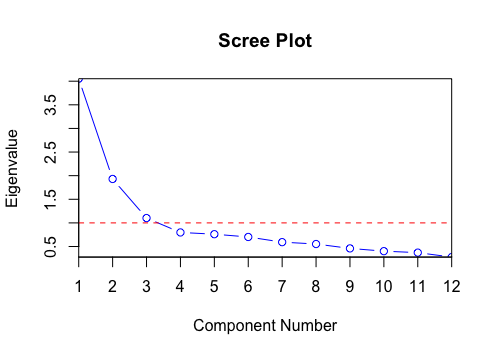
\includegraphics[width=4in]
{pca/scree.png}
\caption{Scree plot. (from Wikipedia entry \qt{Scree plot})
For a geologist, a scree is the edge of a cliff. It looks just like the blue 
curve in this figure, like a decaying exponential.}
\label{fig-scree}
\end{figure}

\item {\bf Plots}

This section is based on Ref.\cite{wiki-biplot}.

Suppose 

\beq
X= U\Lam W^T=\sum_{f=0}^{\calf}\lam_f u_f w_f^T
\eeq
where $\lam_f\in \RR$, $u_f\in \RR^{N\times 1}$
and $w_f\in \RR^{\calf\times 1}$. 
 
 
Suppose the unit column vectors $w_1,
w_2\in\RR^{\calf\times 1}$
are the first two PA, and $\lam_1^2, \lam_2^2$ are the corresponding PVs.

{\bf PC scores} are defined as

\beq
\left(
\frac{(Xw_1)_\s}{\sqrt{\lam_1}},
\frac{(Xw_2)_\s}{\sqrt{\lam_2}}\right)
=  (\sqrt{\lam_1}(u_1)_\s,\sqrt{\lam_2}(u_2)_\s) 
\eeq
for all data points $\s$.


Let $e_f\in \RR^{\calf\times 1}$ 
be a one hot vector with 1 at position $f=1,2 \dots, \calf$.


The {\bf loadings} (i.e., weights) are defined as

\beq
(\sqrt{\lam_1}e_f^T w_1, \sqrt{\lam_2}e_f^T w_2)=
(\sqrt{\lam_1}(w_1)_f, \sqrt{\lam_2}(w_2)_f)
\eeq
for all features $f$.

Fig.\ref{fig-scree} is a plot of the
PVs $\lam_i^2$ versus $i$. Such a plot is 
called a {\bf scree plot}.

Fig.\ref{fig-scores-loadings-biplot}
shows three types of plots: a {\bf PC scores plot}, a {\bf loadings plot}, and a biplot. A {\bf biplot} is a superposition
of the PC scores plot and the loadings plot.



\begin{figure}[h!]
\centering
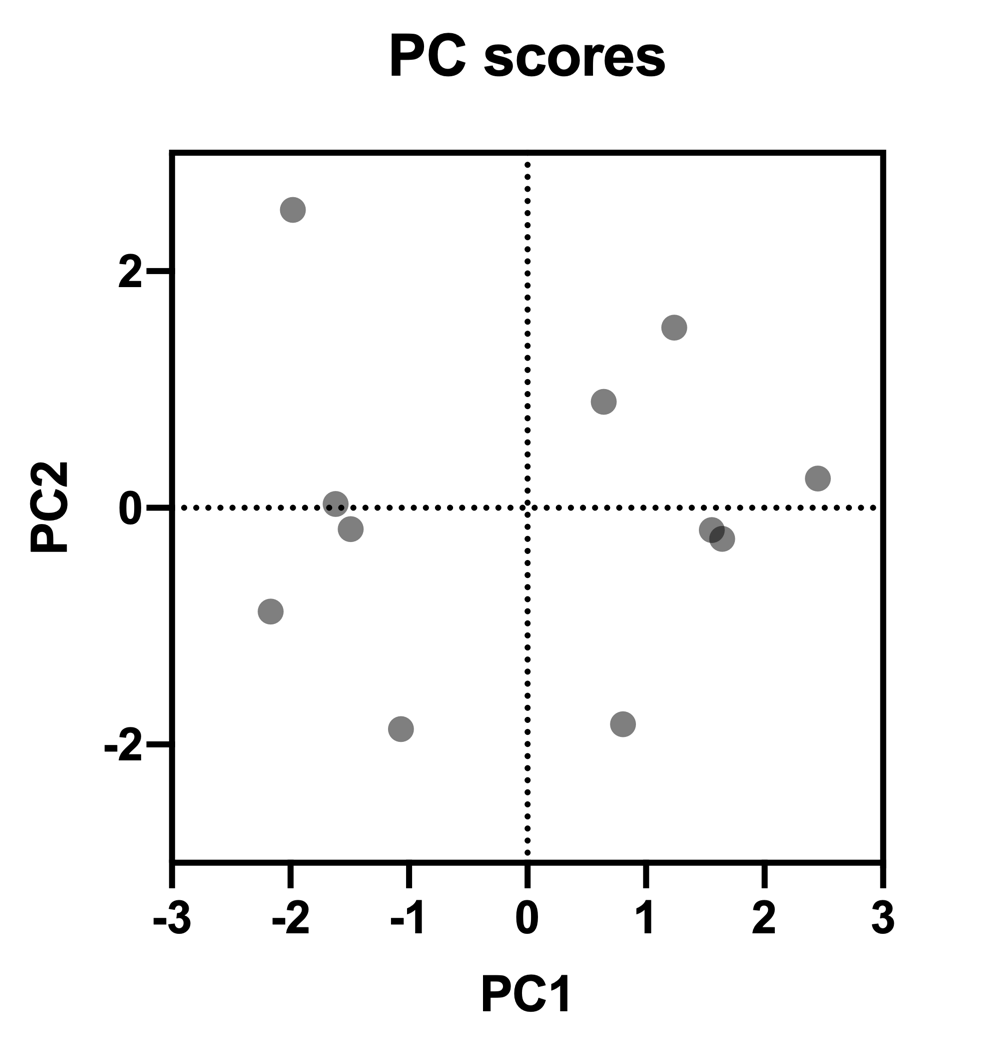
\includegraphics[width=2.5in]
{pca/pc-scores.png}
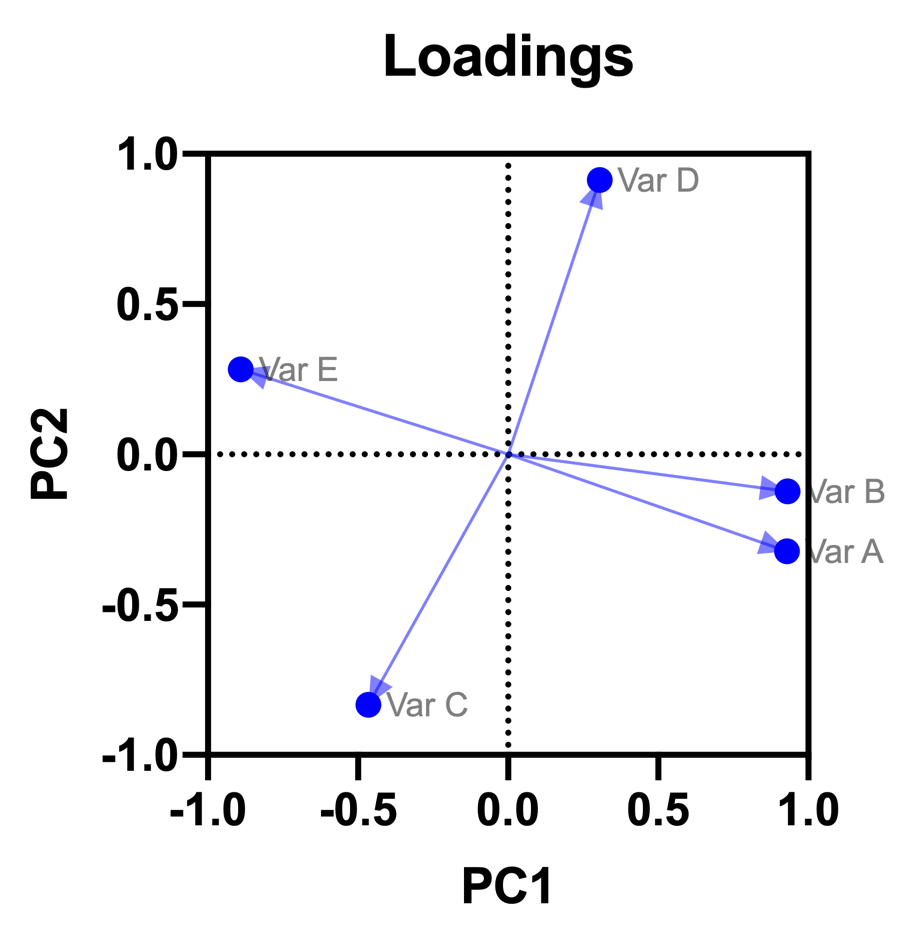
\includegraphics[width=2.5in]
{pca/loadings.png}
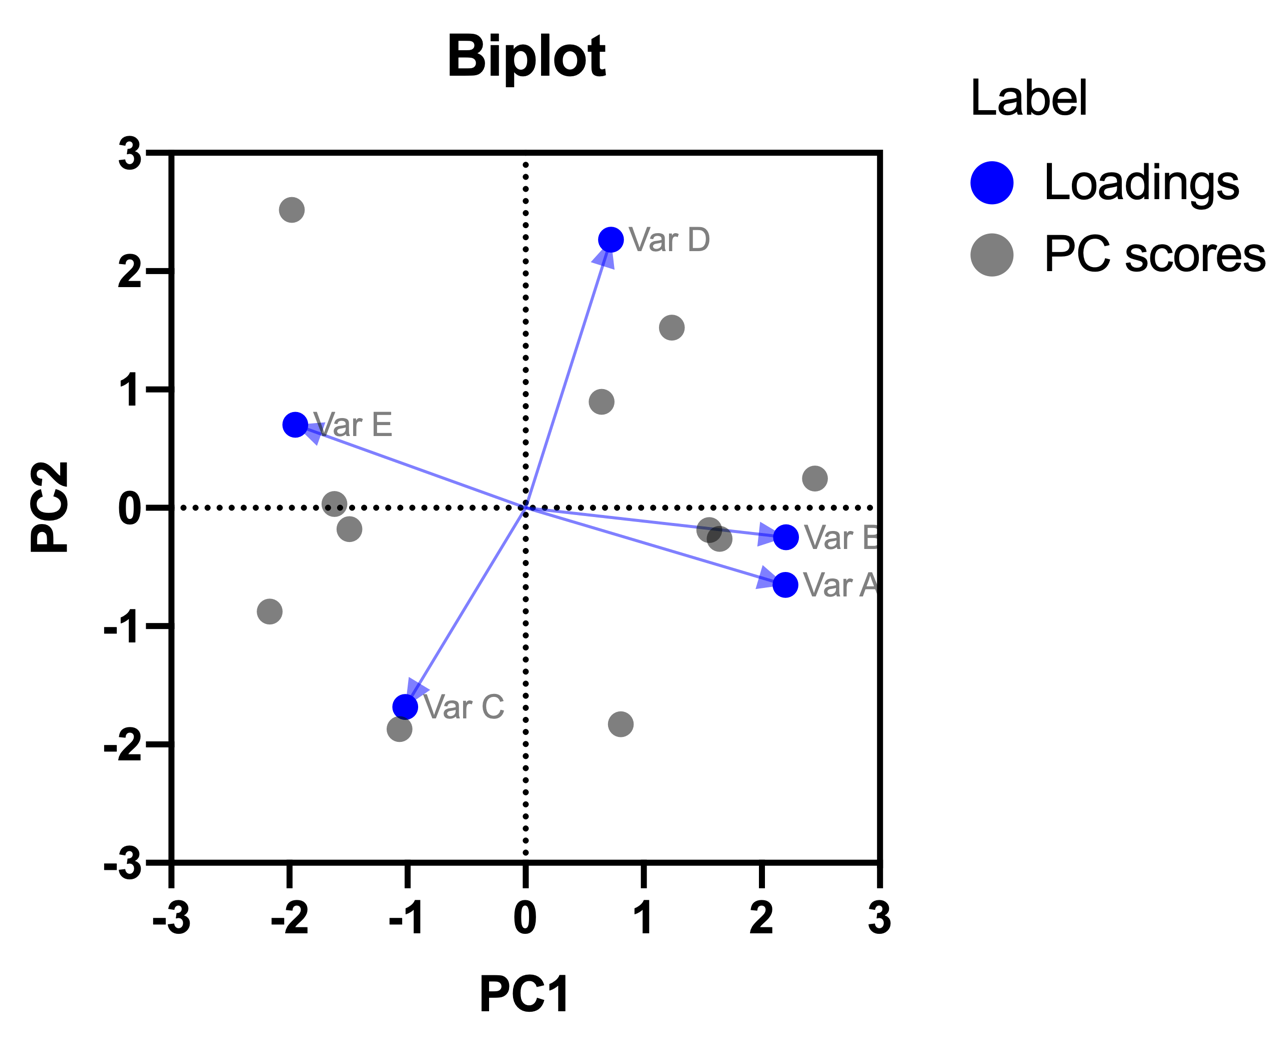
\includegraphics[width=4.5in]
{pca/biplot.png}

\caption{PC scores plot, loadings plot, and biplot. (from the documentation for the Prism software made by graphpad.com)}
\label{fig-scores-loadings-biplot}
\end{figure}




\end{itemize}
